\documentclass[a4paper,12pt]{article}
\author{Adam Ilyas 725819}
\title{
CS-E5740 Complex Networks, \\
Answers to exercise set 2
}

\usepackage{amsfonts}
\usepackage{verbatim}
\usepackage{amsmath}
\usepackage{amsfonts}
\usepackage{graphicx}
\usepackage[english]{babel}
\usepackage{listings}

\begin{document}
\vspace{8pt}

\maketitle

Acknowledgements: Lukas Haug, Bianca Lachennmann, Christoph Berger, Zeyneb Erdogan
\section{Ensemble averages by enumeration}

Graph ensembles are distributions of graphs, where each graph
$G_i$ has a certain probability $\pi_i$.
The ensemble average of a quantity X is defined as $\langle X \rangle = \sum_i\pi_iX(G_i)$.
Note that this is the expected value of X across the ensemble.
Let us define following quantities: $k(G)$ is the average
degree of the graph $G$, $c(G)$ is the average clustering coefficient for graph G (assuming that the
clustering coefficient gets value 0 for nodes of degree 0 and 1), and $d^*(G)$ is the diameter of the
connected component of the graph G that has the largest diameter.



\begin{minipage}{\linewidth}
\centering
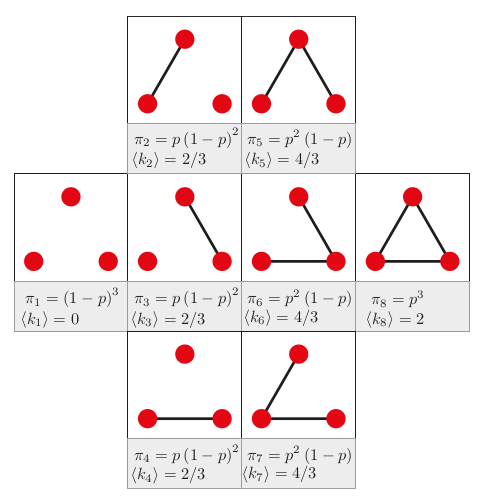
\includegraphics[width=7cm]{assets/ensemble.png}
\end{minipage}

\begin{minipage}{\linewidth}
  \centering
  \begin{tabular}{c|c|c|c|c}
    Ensemble\\i & Probability  & Average Degree & Cluster Coefficient & Diameter\\
    \hline
    1 & $(1-p)^3$ & 0 & 0 & 0\\
    2 & $p(1-p)^2$ & 2/3 & 0 & 1\\
    3 & $p(1-p)^2$ & 2/3 & 0 & 1 \\
    4 & $p(1-p)^2$ & 2/3 & 0 & 1 \\
    5 & $p^2(1-p)$ & 4/3 & 0 & 2 \\
    6 & $p^2(1-p)$ & 4/3 & 0 & 2 \\
    7 & $p^2(1-p)$ & 4/3 & 0 & 2 \\
    8 & $p^3$ & 2 & 1 & 1
\end{tabular}     
\end{minipage}

\begin{itemize}

  
\item[a) ] Calculate, using pen and paper, $\langle k\rangle$, $\langle c \rangle$, and $\langle  d^* \rangle$ for $G(N=3, p = 1/3)$  in which $N$ is the number of nodes and $p$ is the edge density


\begin{enumerate}
\item Average Degree $\langle k  \rangle$
  \begin{equation}
    \begin{split}
      \langle k\rangle & = \sum_i^N\pi_i \langle k_i \rangle \\
      & = (1 - p)^3 \times 0 + 3p(1-p)^2 \times 2/3 + 3p^2(1-p) \times 4/3 + p^3 \times 2\\
      & = 8/27 + 8/27 + 2/27 = 18/27\\
      & = 2/3  \end{split}
  \end{equation}
\item Average Coefficient $\langle c \rangle: 1/p^3 = 1/27$

\item  $d*(G)$ Diameter  (Furthest path): \\
  $1 \times 4/27 \times 3 + 2 \times 2/27 \times 3 + 1 \times 1/27 = 25/27 $
  
  \end{enumerate}

\item[b) ] Calculate, using pen and paper, the formulas for $\langle k\rangle$, $\langle c \rangle$, and $\langle  d^* \rangle$ for $G(N=3, p)$ (that is, for N = 3 and all possible values of p). Remember to simplify the formulas you
get as results.

\begin{enumerate}
\item Average number of edges $\langle m \rangle = \binom{N}{2}p$\\
  Average degree
  \begin{equation}
    \begin{split}
      \langle k \rangle & = 2 \langle m \rangle / N\\ & = p \times N(N-1)/N \\ & = p \times (N-1) \\ & = p \times 2
    \end{split}
  \end{equation}

\item Average clustering coefficient
  \begin{equation}
    \begin{split}
      \langle c \rangle & = \sum_{i=1}^8\pi_i \times \langle c_i \rangle
      \\ & = p^3
    \end{split}
  \end{equation}

\item Average Diameter
  \begin{equation}
    \begin{split}
      \langle d* \rangle & = \sum_{i=1}^8 \pi_i \times \langle d_i \rangle \\
      & = 1 \times (1-p)^2p \times 3 + 2 \times (1-p)p^2 \times 3 + 1 \times p^3\\
      & = 3p - 2p^3
    \end{split}
  \end{equation}
\end{enumerate}
  
\end{itemize}

\section{Properties of Erdős-Rényi (ER) networks}
Erdős-Rényi networks are random networks where N nodes are randomly connected such that
the probability that a pair of nodes are linked is p. In network science, the ER random graphs
are important because they provide the simplest reference to which one can compare real-world
networks. In this exercise, we will analyze some of the properties of ER graphs.

\begin{itemize}
 \item[a) ] The degree distribution $P(k)$ of ER networks is binomial: $$P(k) = \binom{(N-1)}{k}p^k (1-p)^{(N-1) - k}  $$ where N equals the number of nodes in the network. Explain in detail the origin of each
of the three factors in the above formula. You don’t need to derive the distribution, but it
should be visible from your answer that you understand the meaning of each of the terms.

\begin{enumerate}
\item Each node’s number of links comes
  from N-1 independant trials where each trial has the probability p of success)
\item If there are k successes (k neighbours), there are N-1-k 'failures' (failed links), where each failure has the probability 1-p.

\item Since for N-1 trials, there can be $\binom{N-1}{k}$ combination of k success and N-1-k failures 
\end{enumerate}

\item[b) ] In ER networks, the expected value of the average clustering coefficient $\langle c \rangle  $ equals
p. Explain, why this is the case.
Hints:
\begin{itemize}
\item[--] What is the expected value of the clustering coefficient for one node?
\end{itemize}
  
Clustering Coefficient for a node can be represented as $$\frac{\# \text{ edges between
    its neighbours}}{\# \text{ possible edges between its neighbours} } $$

Which can also represent the probability of an edge between a node's neighbours. Hence, the average clustering coefficient, can be exactly this probability, since this is true for all nodes.

\item[c) ] Explain, what happens to $ \langle c \rangle $  , if $N \rightarrow \infty$ with     $\langle k \rangle $ bounded.


  \begin{itemize}
  \item[--] Mathematically, if x is ‘bounded’ then x is always smaller than some possibly big, but finite, number M .
  \end{itemize}
  Since clustering coefficient is independant of the total number of Nodes, then the average clustering coefficient  $\langle k \rangle = p$

\item[d) ] Use NetworkX to calculate estimates for the ensemble averages $\langle k \rangle$, $\langle c \rangle$, and $\langle d* \rangle$ defined in the Exercise 1. Do this by generating 100 ER networks for each value of p in
range p = [0.00, 0.05, ..., 0.95, 1] and N = 3. An estimate for the ensemble average hXi
can be calculated for each value of p by calculating the average value of X over the 100
realisations. Plot the quantities, such that p values are on the x-axis and $\langle X \rangle$ values are
on the y-axis. If you solved the part b of Exercise 1, you can check the correctness of your
results by including your analytical solution to these plots. Repeat the same exercise with
N = 100.
  
\begin{minipage}{\linewidth}
\centering
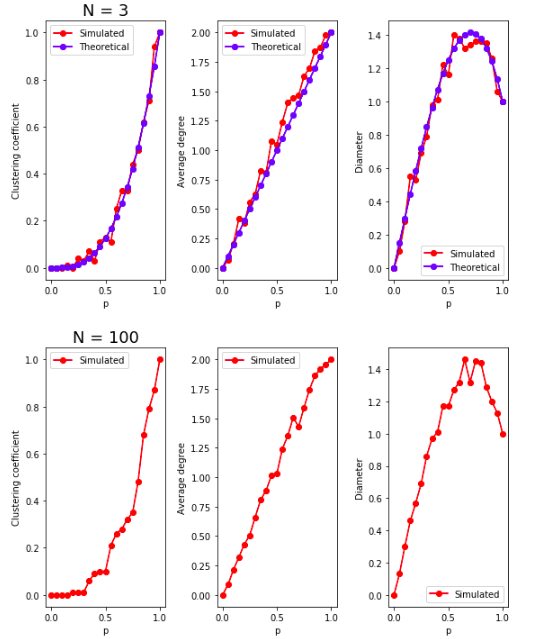
\includegraphics[width=9cm]{assets/question2.png}
\end{minipage}\hfill

  
\end{itemize}

\section{Implementing the Watts-Strogatz small-world model}
In this exercise, you will implement the Watts-Strogatz small-world model [1], which is a very
simple network model that yields small diameter as well as high level of clustering. In practice,
the Watts-Strogatz model is a ring lattice where some of the links have been randomly rewired.
The model has three parameters: network size N , m (each node on the ring connects to m
nearest neighbors both to the left and to the right), and p, the probability of rewiring one end
of each link to a random endpoint node.

\begin{itemize}
\item[a) ] Implement the Watts-Strogatz small world model and visualize the network
using N = 15, m = 2 p = 0.1, and N = 100, m = 2 p = 0.05 using a circular layout algorithm 
nx.draw\_circular , and check that the networks look right. For each network Re-
port the total number of links and also the number of rewired links.

\begin{lstlisting}
def ws(n, m, p):

network = ring(n, m)
    all_edges = list(network.edges()) # same as copy
    
    rewired_num = 0 # tracks the number of rewired links
    total_num = len(all_edges)
    
    for edges in all_edges:
        if np.random.rand() < p:
            rewired_num += 1
            # rewire
            u, v = edges
            network.remove_edge(u, v)
            other_node = random.choice(
                list(nx.non_neighbors(network, u))
            )
            network.add_edge(u, other_node)
            
    print("total number of links:")
    print(total_num)
    print("number of rewired links:")
    print(rewired_num)
    return network

\end{lstlisting}
\begin{minipage}{0.5\linewidth}
\centering
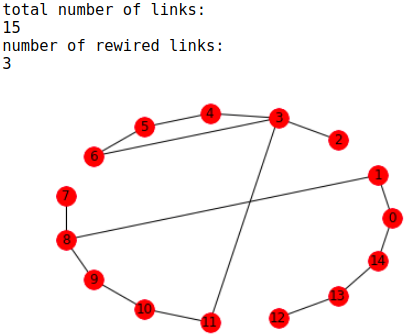
\includegraphics[width=6cm]{assets/rewire1.png}
\end{minipage}\hfill
\begin{minipage}{0.5\linewidth}
\centering
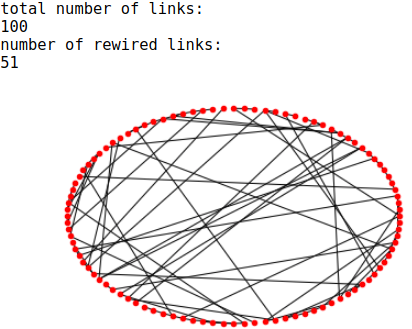
\includegraphics[width=6cm]{assets/rewire2.png}
\end{minipage}

\item[b) ] Plot the relative average clustering coefficient c(p)/c(p = 0) and average shortest
path length l(p)/l(p = 0) vs. p in your network, for p = 0.001, . . . , 1.0 (see template for
the log-spaced values). Here, relative=average value for given p divided by the same value
for p = 0. Use N = 500 and m = 2. Use a logarithmic x-axis in your plot (ax.semilogx).
Check that your results are in line with the plots in the lecture slides.

\begin{minipage}{\linewidth}
\centering
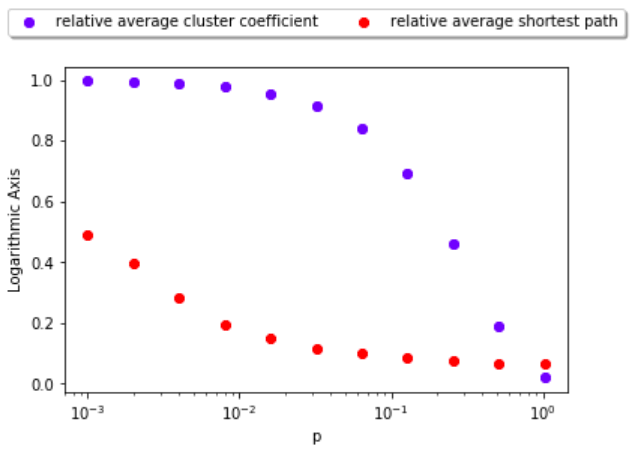
\includegraphics[width=12cm]{assets/relative.png}
\end{minipage}\hfill
\end{itemize}
\end{document}